%%%%%%%%%%%%%%%%%%%%%%%%%%%%%%%%%%%%%%%%%
% Beamer Presentation
% LaTeX Template
% Version 1.0 (10/11/12)
%
% This template has been downloaded from:
% http://www.LaTeXTemplates.com
%
% License:
% CC BY-NC-SA 3.0 (http://creativecommons.org/licenses/by-nc-sa/3.0/)
%
%%%%%%%%%%%%%%%%%%%%%%%%%%%%%%%%%%%%%%%%%

%----------------------------------------------------------------------------------------
%	PACKAGES AND THEMES
%----------------------------------------------------------------------------------------

%\documentclass[UTF8,aspectratio=169,14pt]{ctexbeamer}
\documentclass[UTF8,aspectratio=169]{ctexbeamer}
\usepackage{hyperref}
\hypersetup{
	colorlinks=true,
	linkcolor=red,
	anchorcolor=blue,
	citecolor=green
}

\mode<presentation> {
	
	% The Beamer class comes with a number of default slide themes
	% which change the colors and layouts of slides. Below this is a list
	% of all the themes, uncomment each in turn to see what they look like.
	
	%\usetheme{default}
	%\usetheme{AnnArbor}
	%\usetheme{Antibes}
	%\usetheme{Bergen}
	%\usetheme{Berkeley}
	%\usetheme{Berlin}
	%\usetheme{Boadilla}
	%\usetheme{CambridgeUS}
	%\usetheme{Copenhagen}
	%\usetheme{Darmstadt}
	%\usetheme{Dresden}
	%\usetheme{Frankfurt}
	%\usetheme{Goettingen}
	%\usetheme{Hannover}
	%\usetheme{Ilmenau}
	%\usetheme{JuanLesPins}
	%\usetheme{Luebeck}
	\usetheme{Madrid}
	%\usetheme{Malmoe}
	%\usetheme{Marburg}
	%\usetheme{Montpellier}
	%\usetheme{PaloAlto}
	%\usetheme{Pittsburgh}
	%\usetheme{Rochester}
	%\usetheme{Singapore}
	%\usetheme{Szeged}
	%\usetheme{Warsaw}
	
	% As well as themes, the Beamer class has a number of color themes
	% for any slide theme. Uncomment each of these in turn to see how it
	% changes the colors of your current slide theme.
	
	%\usecolortheme{albatross}
	%\usecolortheme{beaver}
	%\usecolortheme{beetle}
	%\usecolortheme{crane}
	%\usecolortheme{dolphin}
	%\usecolortheme{dove}
	%\usecolortheme{fly}
	%\usecolortheme{lily}
	%\usecolortheme{orchid}
	%\usecolortheme{rose}
	%\usecolortheme{seagull}
	%\usecolortheme{seahorse}
	%\usecolortheme{whale}
	%\usecolortheme{wolverine}
	
	%\setbeamertemplate{footline} % To remove the footer line in all slides uncomment this line
	%\setbeamertemplate{footline}[page number] % To replace the footer line in all slides with a simple slide count uncomment this line
	
	%\setbeamertemplate{navigation symbols}{} % To remove the navigation symbols from the bottom of all slides uncomment this line
}

\usepackage{graphicx} % Allows including images
\graphicspath{{./figs/}}
\usepackage{booktabs} % Allows the use of \toprule, \midrule and \bottomrule in tables
\usepackage{longtable}
\usepackage{listings}
\usepackage{xcolor}
\lstset{numbers=left, %设置行号位置
	numberstyle=\tiny, %设置行号大小
	keywordstyle=\color{blue}, %设置关键字颜色
	commentstyle=\color[cmyk]{1,0,1,0}, %设置注释颜色
	frame=single, %设置边框格式
	escapeinside=``, %逃逸字符(1左面的键),用于显示中文
	%breaklines, %自动折行
	extendedchars=false, %解决代码跨页时,章节标题,页眉等汉字不显示的问题
	xleftmargin=2em,xrightmargin=2em, aboveskip=1em, %设置边距
	tabsize=4, %设置tab空格数
	showspaces=false %不显示空格
}
% Fonts
% \usepackage{libertine}
% \setmonofont{Courier}
\setCJKsansfont[ItalicFont=Noto Serif CJK SC Black, BoldFont=Noto Sans CJK SC Black]{Noto Sans CJK SC}
\setmainfont[Ligatures={Common,TeX}]{Linux  Libertine O}
\setmonofont[SmallCapsFont={Latin Modern Mono Caps}]{Latin Modern Mono Light}
\setsansfont{Linux Biolinum O}

\logo{
\includegraphics[width=0.55cm,height=0.55cm]{../../thcs-logo.png}}

%----------------------------------------------------------------------------------------
%	TITLE PAGE
%----------------------------------------------------------------------------------------

\title[第2讲]{第2讲 :OS Architecture \& Structure} % The short title appears at the bottom of every slide, the full title is only on the title page
\subtitle{第七节:Twizzer: OS for Non-Volatile Memory }
\author{陈渝} % Your name
\institute[清华大学] % Your institution as it will appear on the bottom of every slide, may be shorthand to save space
{
	清华大学计算机系 \\ % Your institution for the title page
	\medskip
	\textit{yuchen@tsinghua.edu.cn} % Your email address
}
\date{\today} % Date, can be changed to a custom date


\begin{document}

\begin{frame}
\titlepage % Print the title page as the first slide
\end{frame}

%\begin{frame}
%\frametitle{提纲} % Table of contents slide, comment this block out to remove it
%\tableofcontents % Throughout your presentation, if you choose to use \section{} and \subsection{} commands, these will automatically be printed on this slide as an overview of your presentation
%\end{frame}
%
%%----------------------------------------------------------------------------------------
%%	PRESENTATION SLIDES
%%----------------------------------------------------------------------------------------
%
%%------------------------------------------------
%\section{第一节:课程概述} % Sections can be created in order to organize your presentation into discrete blocks, all sections and subsections are automatically printed in the table of contents as an overview of the talk
%%------------------------------------------------
%-------------------------------------------------
\begin{frame}[plain]
	\frametitle{Recap}
	
	
	
	\begin{columns}
		
		\begin{column}{.6\textwidth}
			
			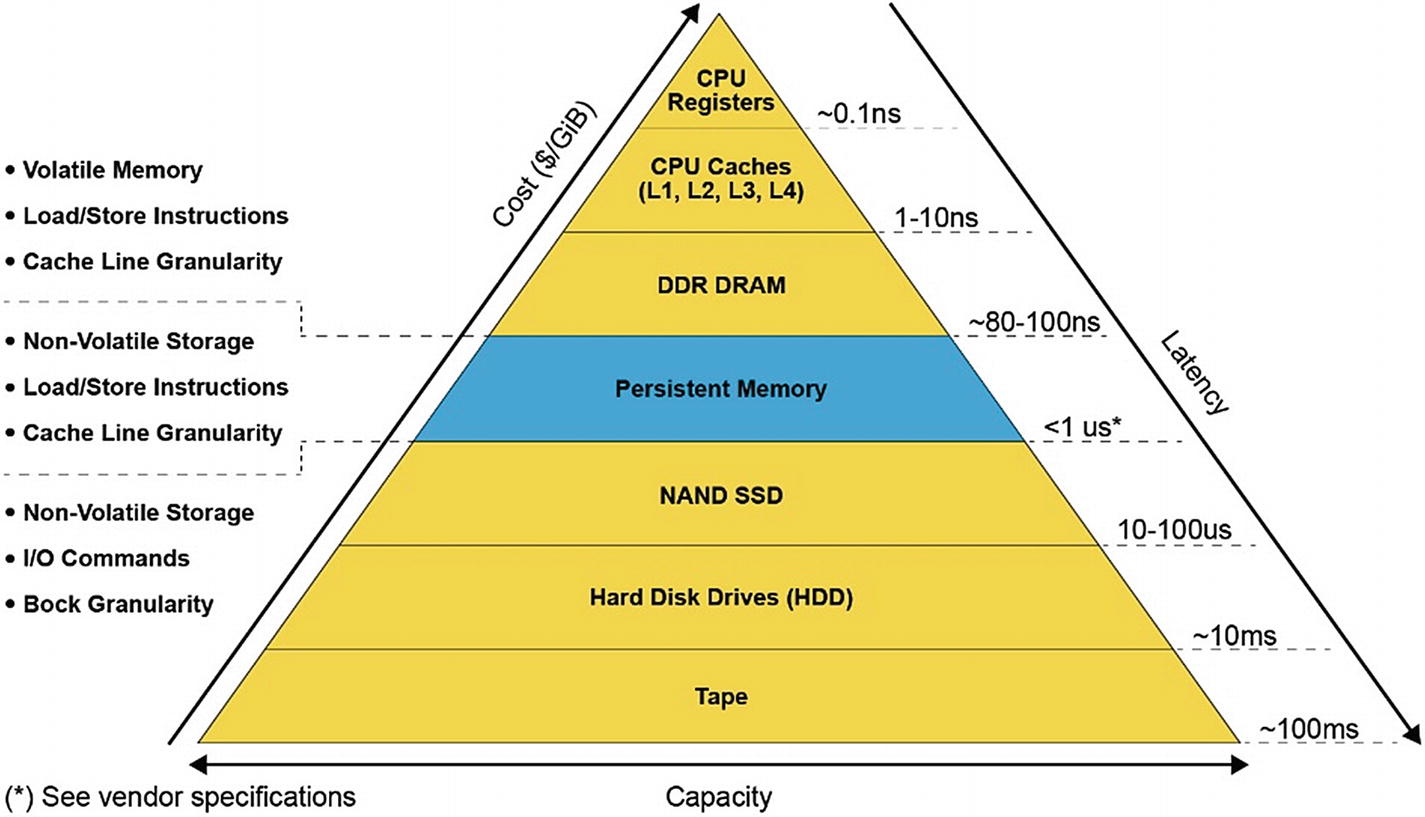
\includegraphics[width=1.\textwidth]{mem-levels}
			
		\end{column}
		
		\begin{column}{.4\textwidth}
			
			
			Hardware Trends on Memory and Storage
			\begin{itemize}
				\item  Non-Volatile Memory
				\begin{itemize}
					\item Growing, becoming persistent
				\end{itemize}
			
				\item Disk or SSD
				\begin{itemize}
					\item Cannot compute on directly
                    \item Access through FileSystem
				\end{itemize}
			\end{itemize}	
			
%			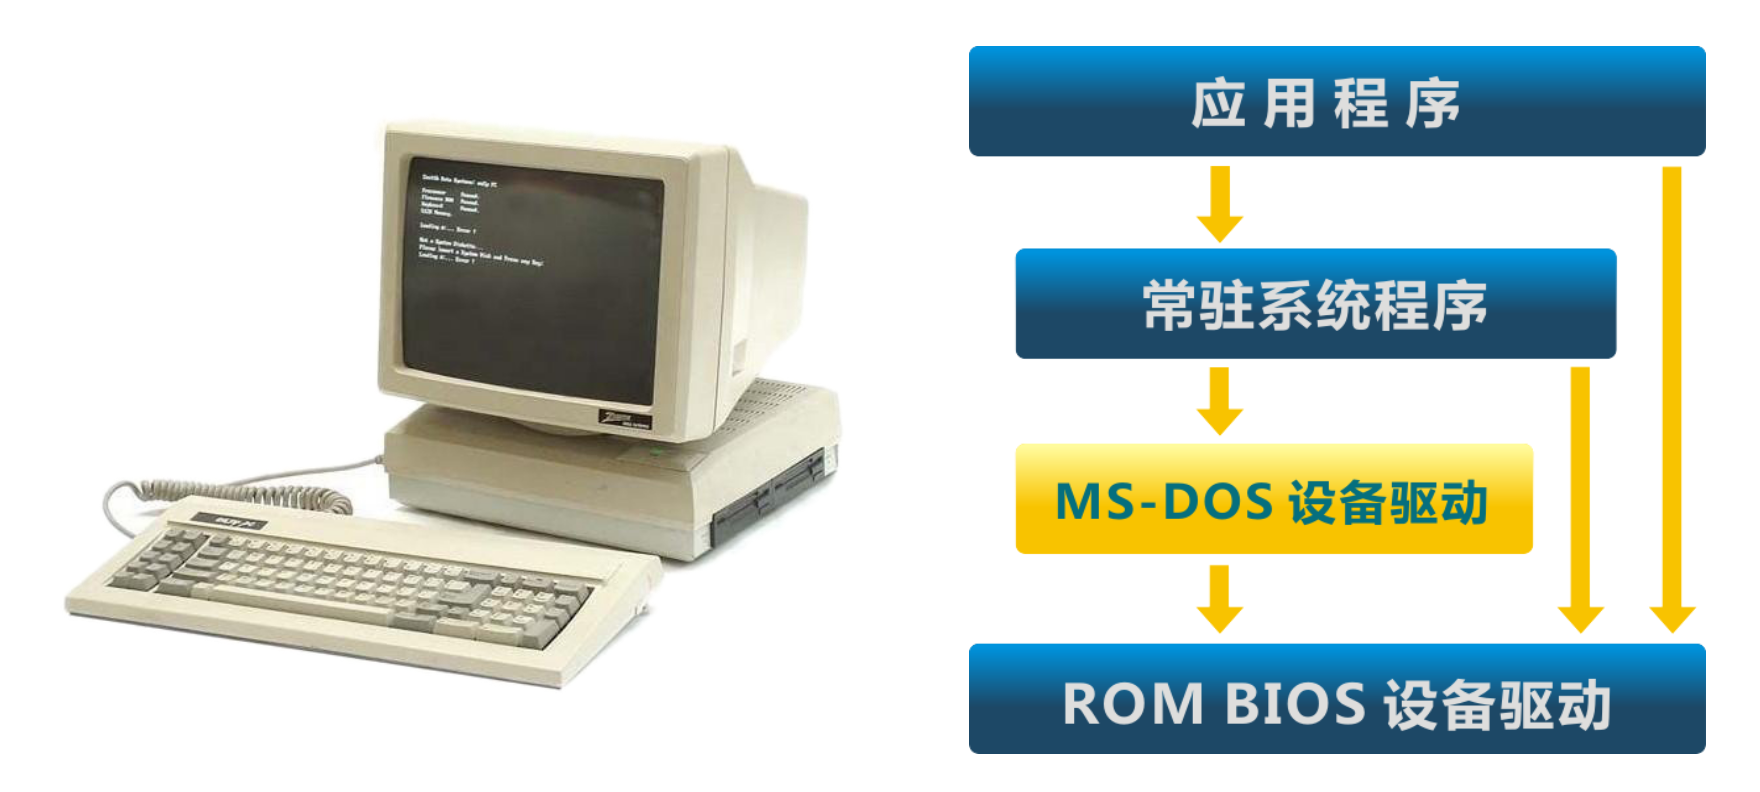
\includegraphics[width=1.\textwidth]{msdos}		
		\end{column}
		
		
	\end{columns}
	
	
\end{frame}

%-------------------------------------------------
\begin{frame}[plain]
	\frametitle{Recap}



	\begin{columns}

	\begin{column}{.5\textwidth}
	
	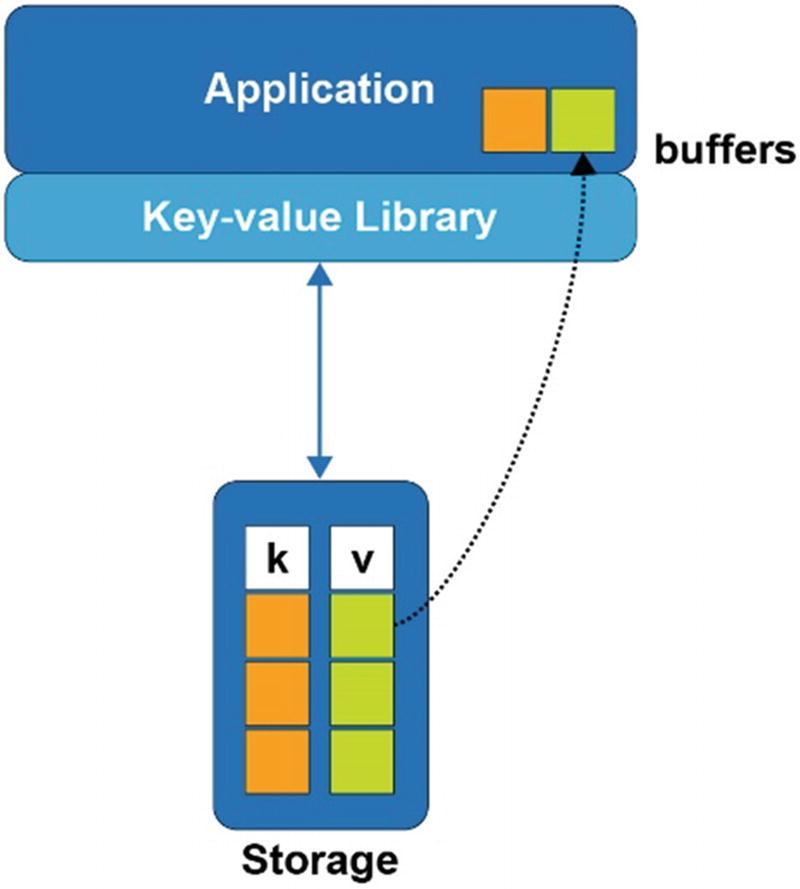
\includegraphics[width=.8\textwidth]{storage-access}
	
	\end{column}

	\begin{column}{.5\textwidth}
	

	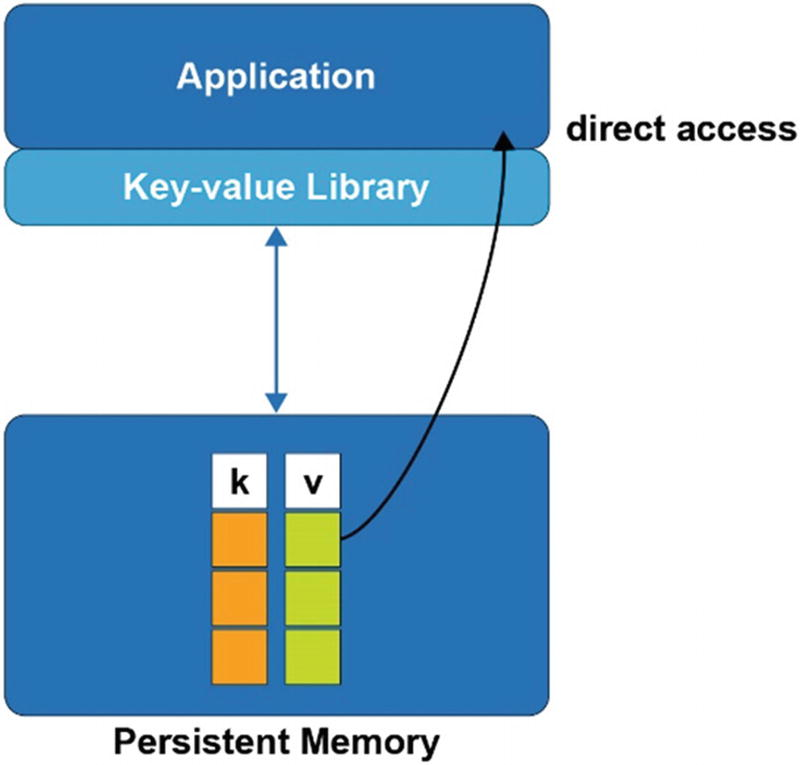
\includegraphics[width=.8\textwidth]{nvm-access}		
	\end{column}
	

\end{columns}


\end{frame}


%-------------------------------------------------
\begin{frame}[plain]
	\frametitle{Recap}
	
	
	
			
	\begin{columns}
    
    \begin{column}{.5\textwidth}
        
        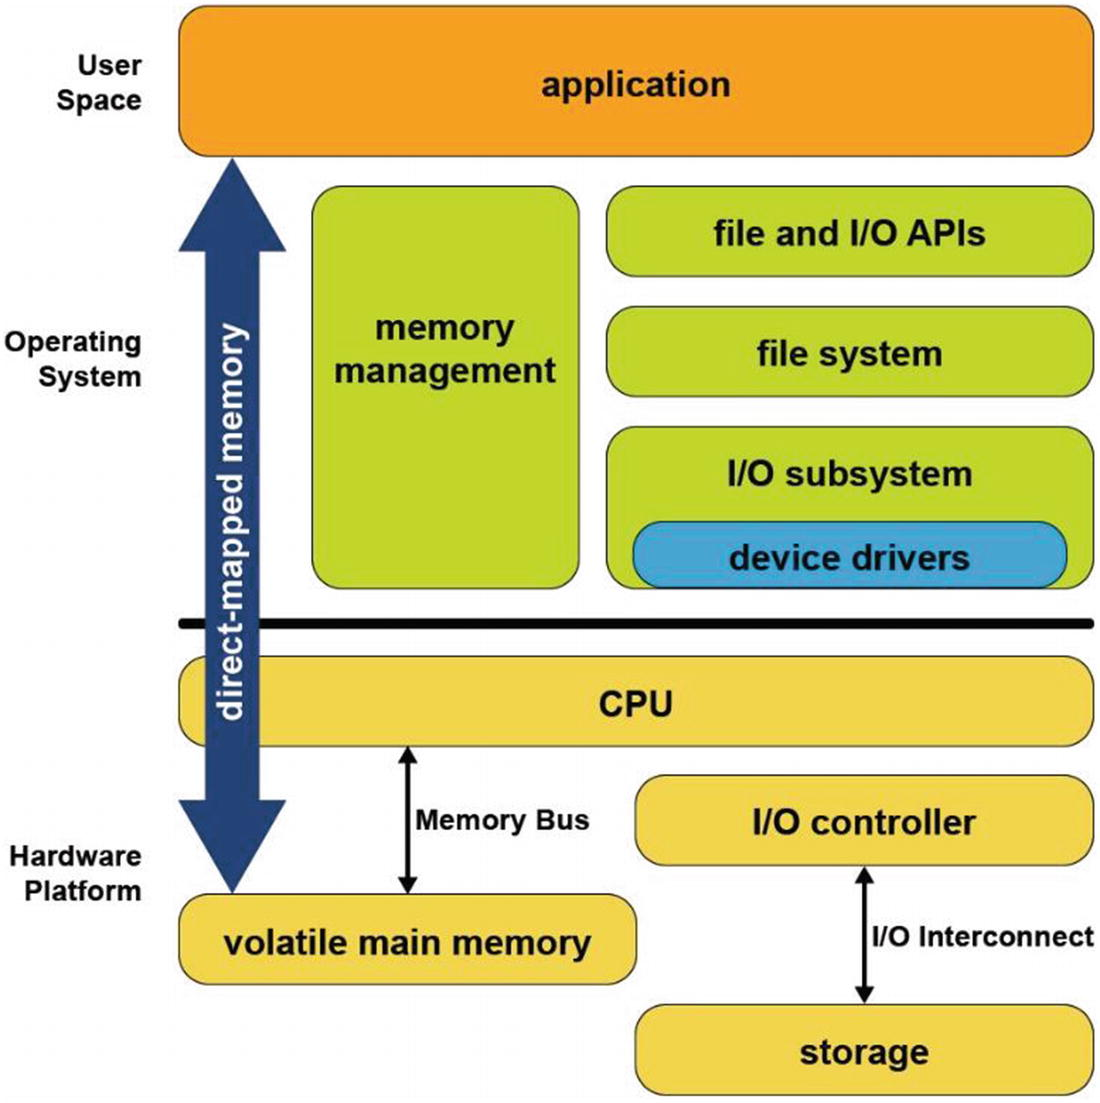
\includegraphics[width=.8\textwidth]{os-with-nvm}
        
    \end{column}
    
    \begin{column}{.5\textwidth}
        
        \Large
        Operating System Support for Memory and Storage	
        \begin{itemize}

            \item operating system manages the mapping

        \end{itemize}	
        		
    \end{column}
    
    
\end{columns}		

	
	
\end{frame}

%-------------------------------------------------
\begin{frame}[plain]
	\frametitle{Recap}
	
	
	
	\begin{columns}
		
		\begin{column}{.5\textwidth}
			
			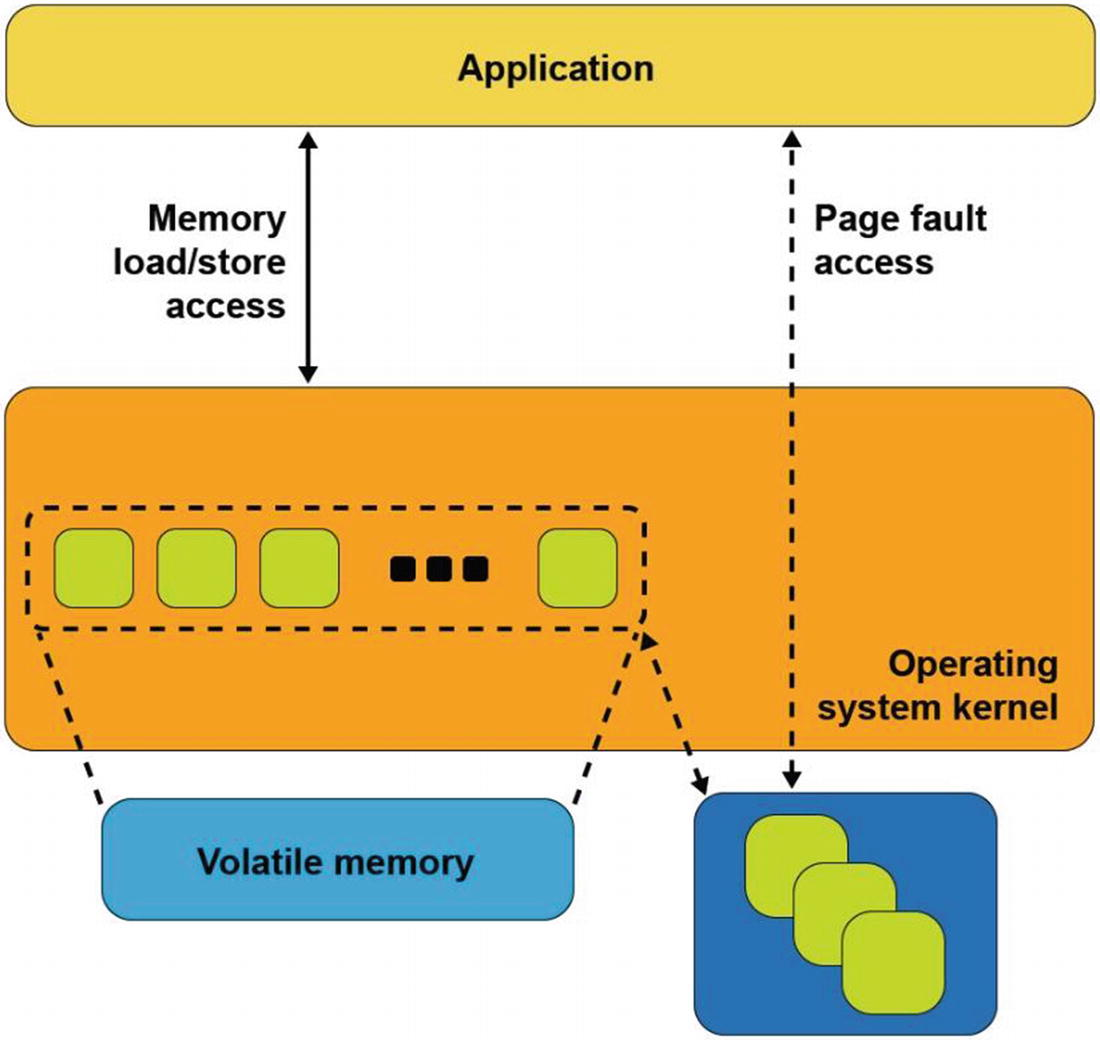
\includegraphics[width=1.\textwidth]{nvm-mmap}
			
		\end{column}
		
		\begin{column}{.5\textwidth}
			
	
			Memory-mapped files with storage
			\begin{itemize}

					\item application calls mmap() on Linux
                    \item page fault exception is raised 
                    \item OS schedules asynchronous I/O operations to write the modifications back 

			\end{itemize}	
			
	
		\end{column}
		
		
	\end{columns}
	
	
\end{frame}

%-------------------------------------------------
\begin{frame}[plain]
	\frametitle{Recap}
	
	
	
	\begin{columns}
		
		\begin{column}{.5\textwidth}
			
			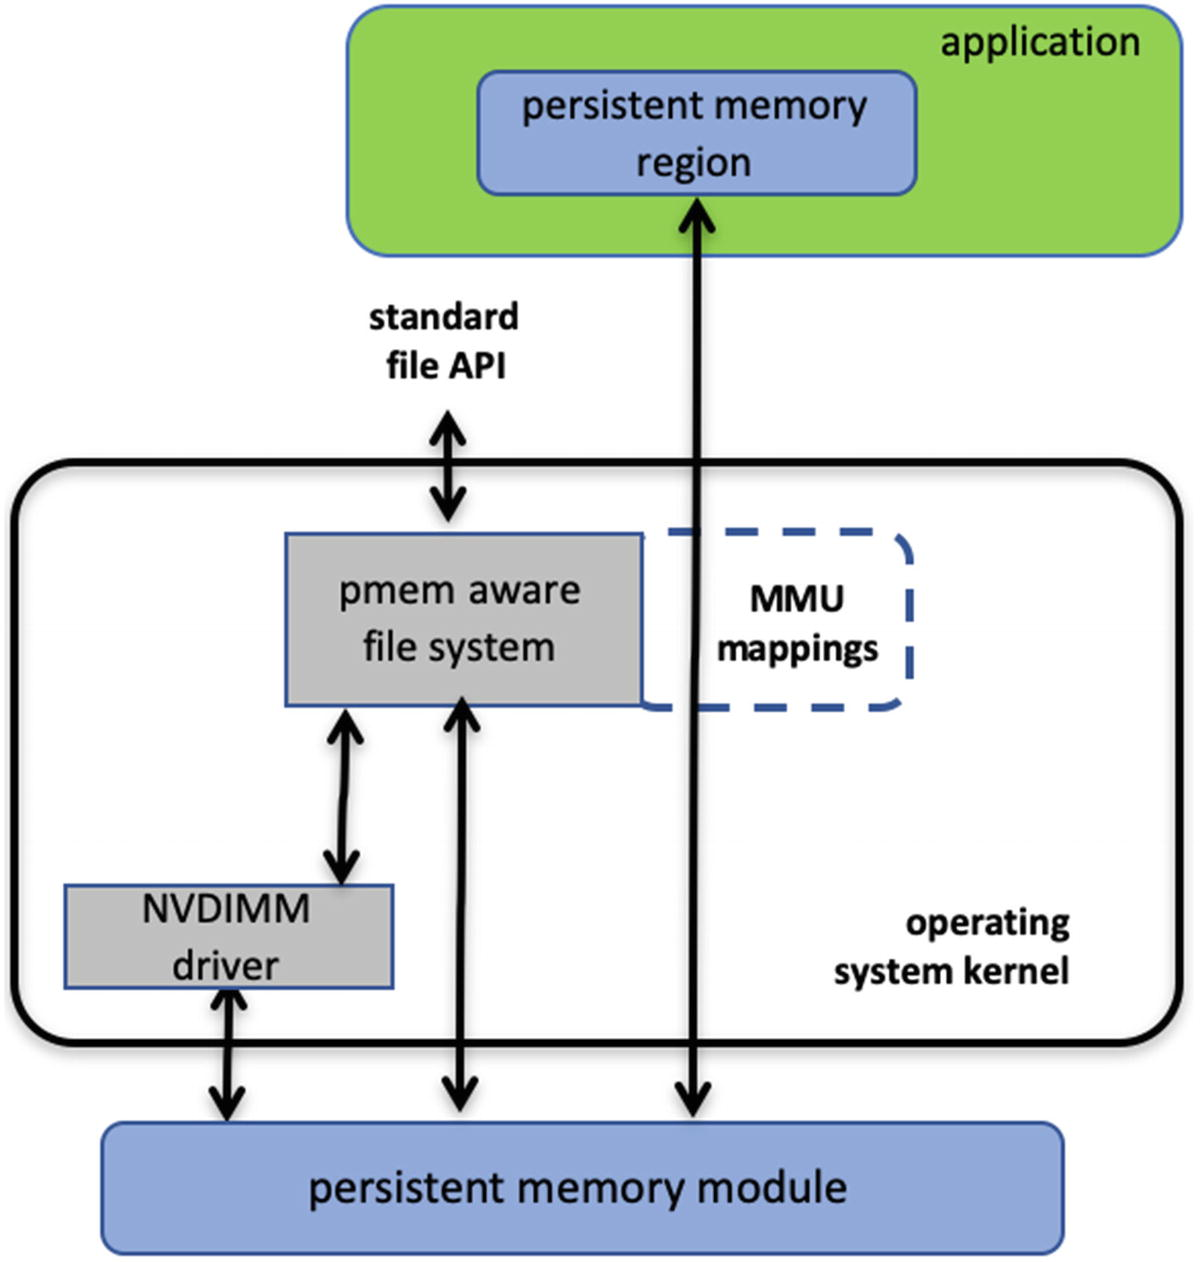
\includegraphics[width=.8\textwidth]{nvm-dax}
			
		\end{column}
		
		\begin{column}{.5\textwidth}
			
			\Large
			Direct access (DAX) I/O and standard file API I/O paths through the kernel	
			\begin{itemize}
                \item libpmem 
			\end{itemize}	
			
		
		\end{column}
		
		
	\end{columns}
	
	
\end{frame}




%-------------------------------------------------
\begin{frame}[plain]
    
    
    
    The complete view of the operating system support NVM
    
    
    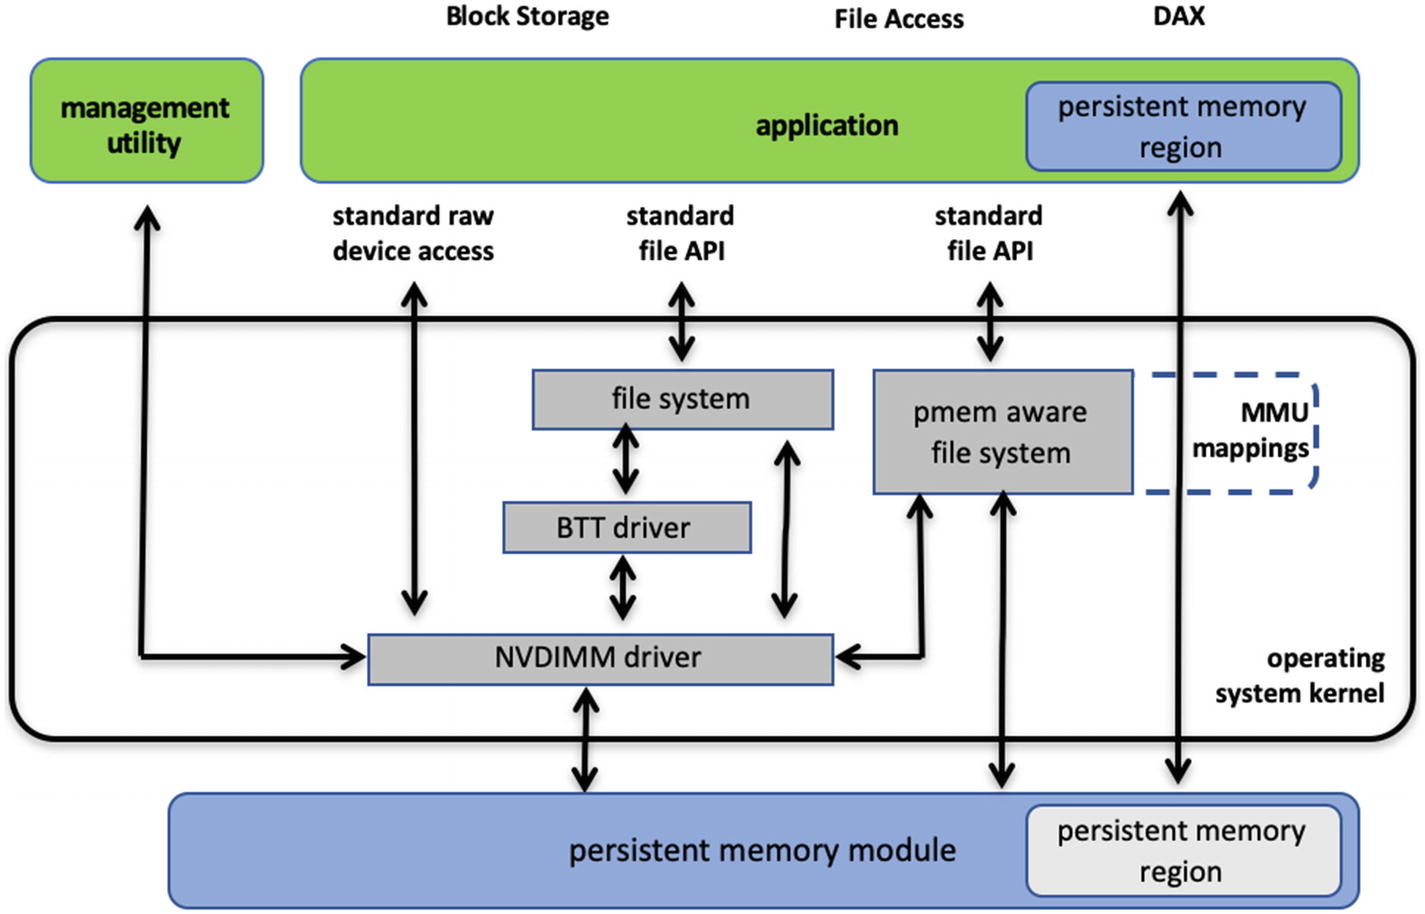
\includegraphics[width=.8\textwidth]{os-with-nvm-overview}
    
    
    
    
\end{frame}

%-------------------------------------------------
\begin{frame}
    
    Persistent Memory in Linux Kernel
    
    \begin{itemize}
        \item PMEM 
        \begin{itemize}
            \item Drives a system physical address range
            \item  Provides direct byte-addressable load/store access 
            \item 'direct\_access’ operation – Translate sector number to Page Frame Number
            \item You can have any DAX-FS on top of it
        \end{itemize}
        \item  Block Window Driver (single DIMM)
        \begin{itemize}
            \item Enables DIMM-bounded failure modes (e.g., RAID)
        \end{itemize}        
    \end{itemize}   
    
    
\end{frame}
%-------------------------------------------------
\begin{frame}
    
    Persistent Memory in Linux Kernel
    
    \begin{itemize}
        \item Block Translation Table (BTT) 
        \begin{itemize}
            \item Sector-sized old device à block translation table 
            \item  On top of whole block device OR a partition of a block device 
            \item Makes every write an “allocating write” i.e., every write goes to a free block. 
        \end{itemize}
        \item Device-DAX
        \begin{itemize}
            \item  Bypass the file system completely
            \item Talks directly to PMEM Namespace
        \end{itemize}    
    \end{itemize}   
    
    
\end{frame}
%-------------------------------------------------
\begin{frame}
    
    Persistent Memory in Linux Kernel
    
    \begin{itemize}
        \item Base Platform
        \begin{itemize}
            \item X86 CPU Instruction:CLFLUSHOPT, CLWB, etc.                    
            \item X86 MM:  Huge Pages – 2MB, GB                        
            \item File System: XFS-DAX, EXT4-DAX                        
        \end{itemize}
    \end{itemize}   
    
    
\end{frame}
%-------------------------------------------------
\begin{frame}
    
    
    
    NVM Prog: Replace read/write calls with memory copy
    
    
    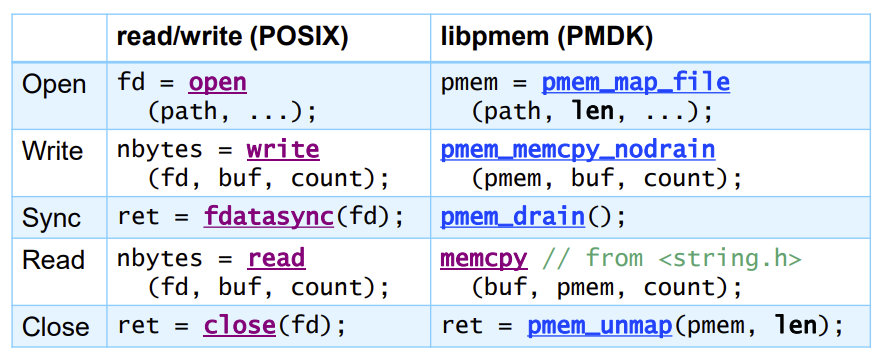
\includegraphics[width=1.\textwidth]{nvm-prog}
    
    
    
    
\end{frame}

%-------------------------------------------------
\begin{frame}
    
    Existing Problems?
    
    \begin{itemize}
    \item POSIX
    \begin{itemize}
        \item Explicit persistence and data access         
        \item Multiple forms of data         
        \item Kernel involvement
        \item  mmap helps, but does not solve the
        virtual memory problem        
    \end{itemize}
    \item  PMDK
    
    \begin{itemize}
        \item No OS support
        \item Data sharing is hard        
        \item Slow pointers        
    \end{itemize}    
\end{itemize}   
    
\end{frame}

%-------------------------------------------------
\begin{frame}

   twizzer OS Overview
       
    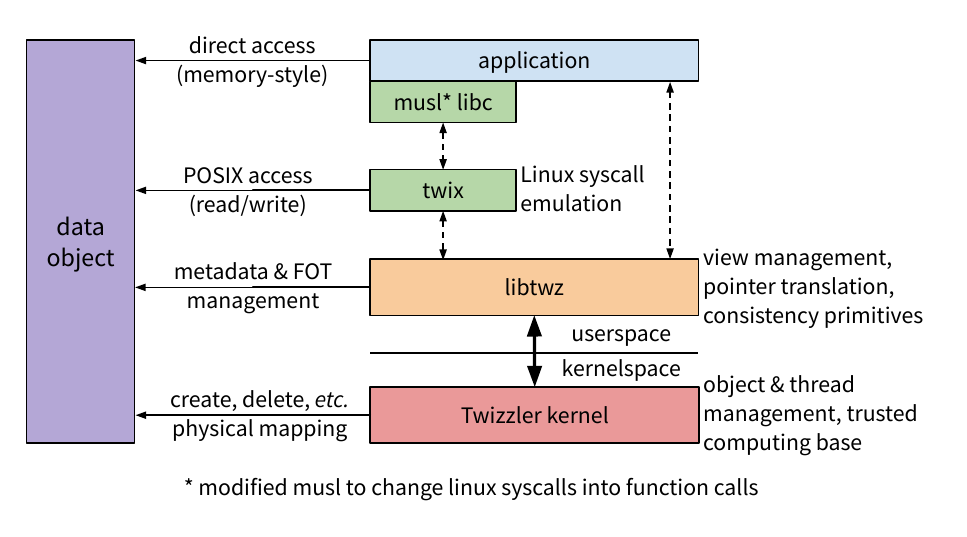
\includegraphics[width=1.\textwidth]{twizzer-overview}

\end{frame}


%-------------------------------------------------
\begin{frame}
    
    Persistent pointers in Twizzler    
    \begin{itemize}
      \item Virtual addresses are the wrong abstraction
    \end{itemize}
    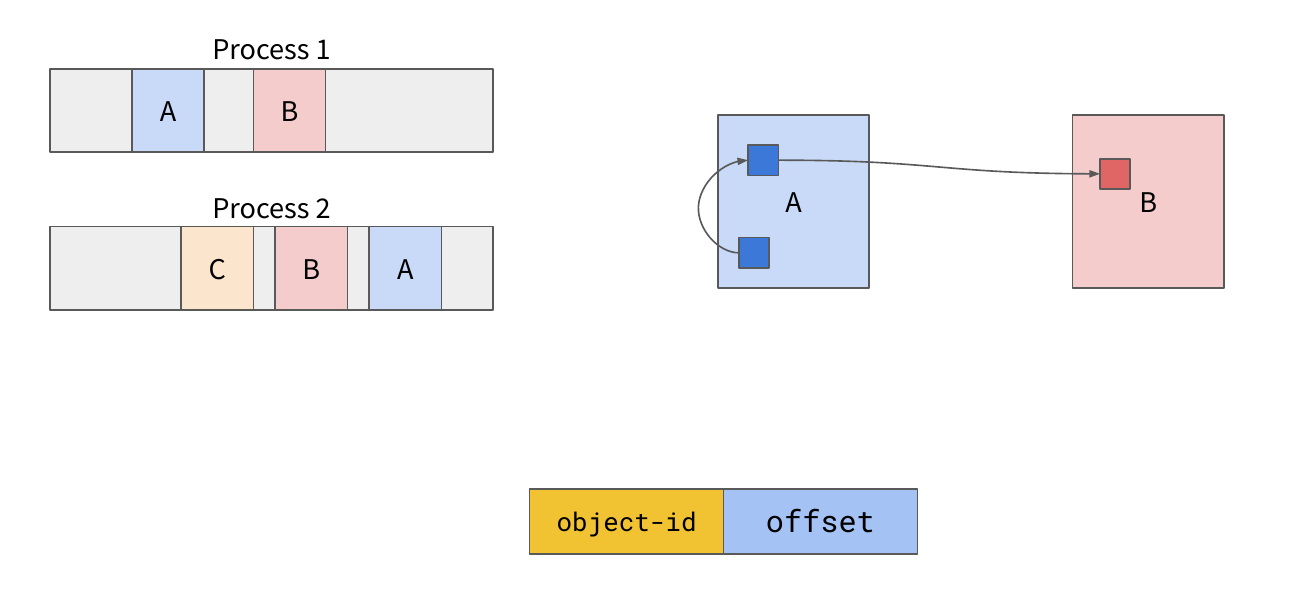
\includegraphics[width=1.\textwidth]{virt-addr}
    
\end{frame}

%-------------------------------------------------
\begin{frame}
    
    Persistent pointers in Twizzler    
    \begin{itemize}
        \item Twizzler’s pointers        
    \end{itemize}
    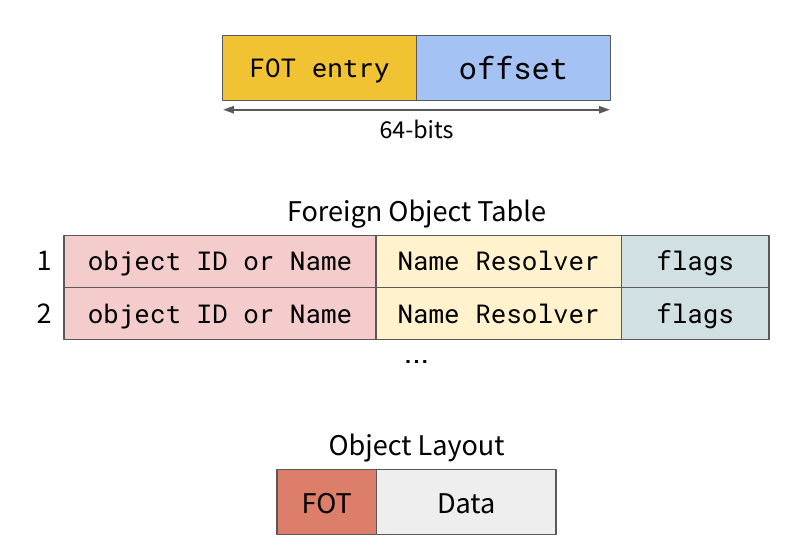
\includegraphics[width=1.\textwidth]{twizzer-pointer}
    
\end{frame}

%-------------------------------------------------
\begin{frame}
    
    Persistent pointers in Twizzler    
    \begin{itemize}
        \item Example pointer resolution
        \item FOT entry of >0 means “cross-object”—points to a different object        
    \end{itemize}
    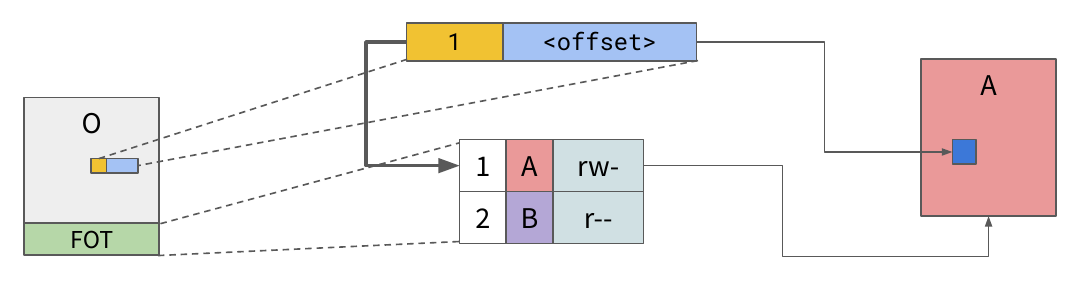
\includegraphics[width=1.\textwidth]{twizzer-pointer-example}
    
\end{frame}

%-------------------------------------------------
\begin{frame}
    
    Persistent pointers in Twizzler    
    \begin{itemize}
        \item Pointer implementation                
    \end{itemize}
    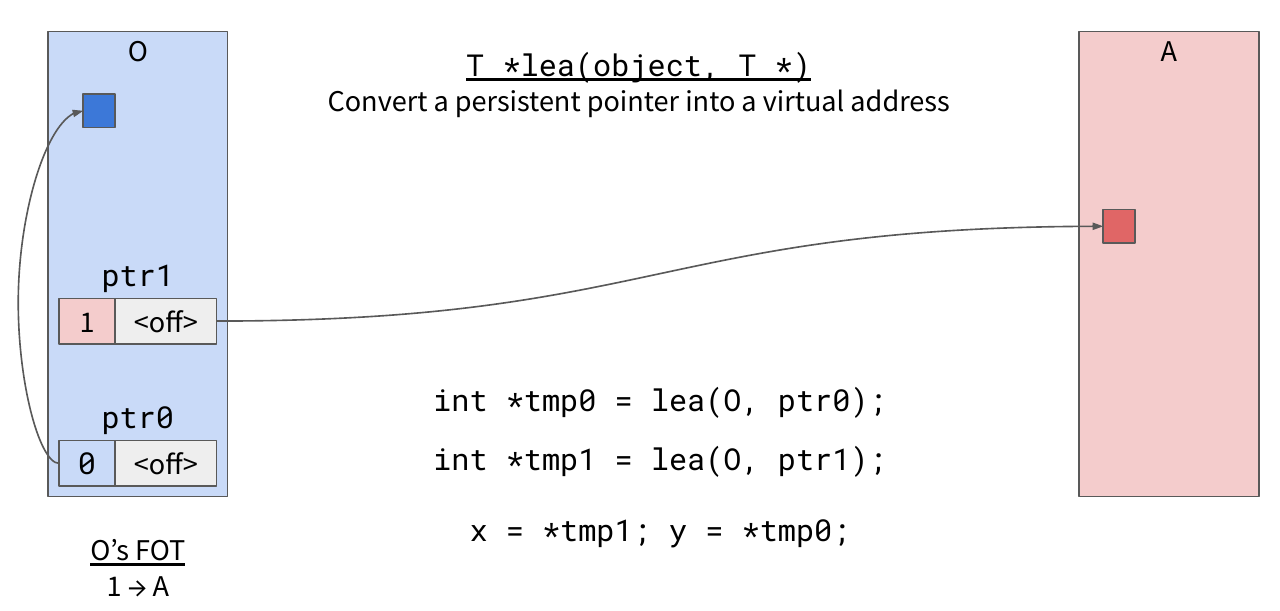
\includegraphics[width=1.\textwidth]{twizzer-pointer-impl}
    
\end{frame}

%-------------------------------------------------
\begin{frame}
    
    Persistent pointers in Twizzler    
    \begin{itemize}
        \item Two-level Mapping                        
    \end{itemize}
    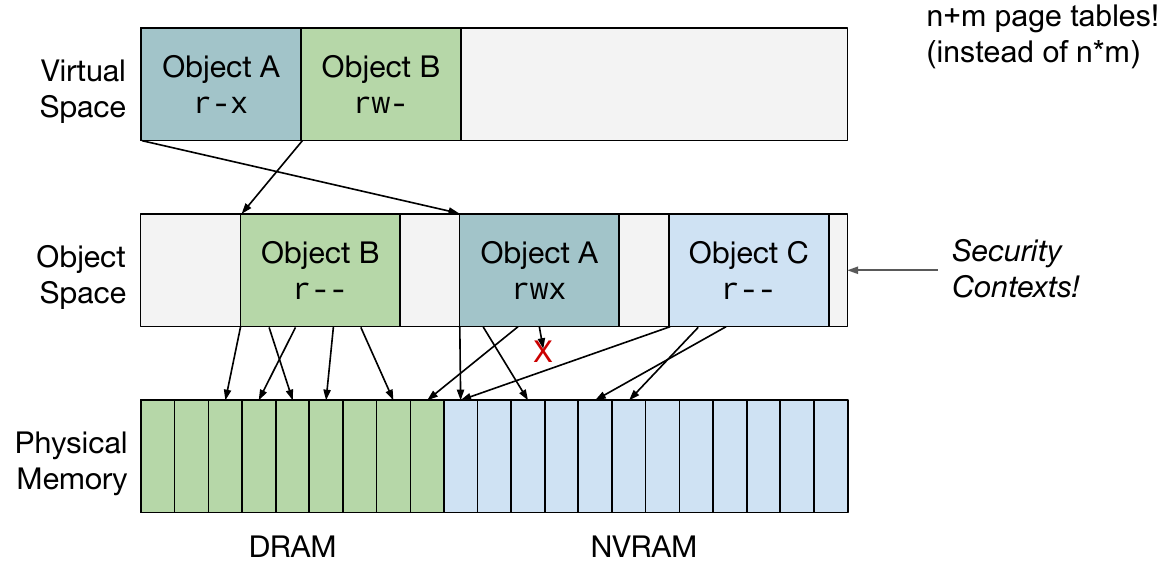
\includegraphics[width=1.\textwidth]{twizzer-pointer-mapping}
    
\end{frame}


%-------------------------------------------------
\begin{frame}
    
    Twizzler in  Venn Diagram    
%    \begin{itemize}
%        \item                                
%    \end{itemize}
    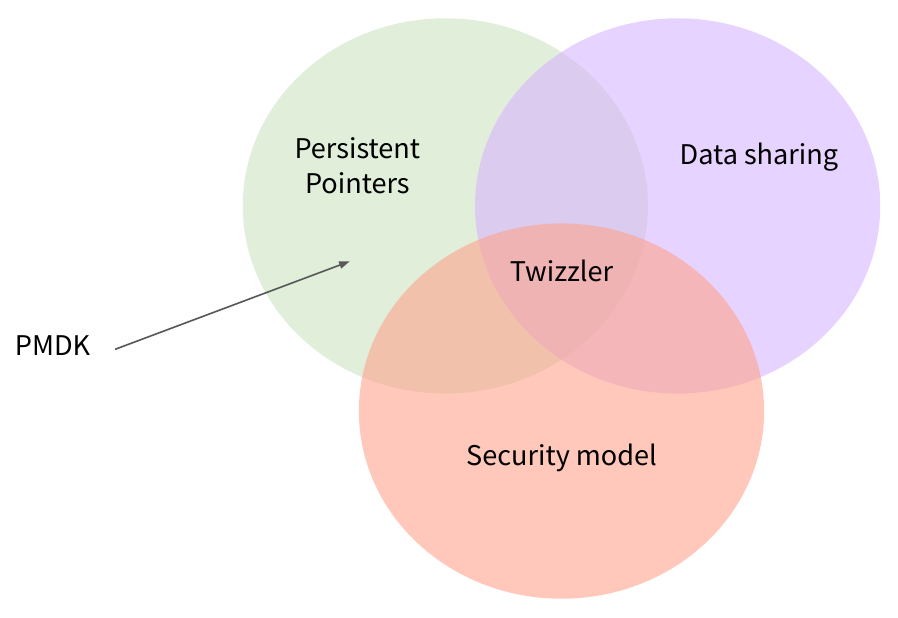
\includegraphics[width=.8\textwidth]{twizzer-venn}
    
\end{frame}

%-------------------------------------------------
\begin{frame}
    
    Benchmark: SQLite, throughput       
    %    \begin{itemize}
    %        \item                                
    %    \end{itemize}
    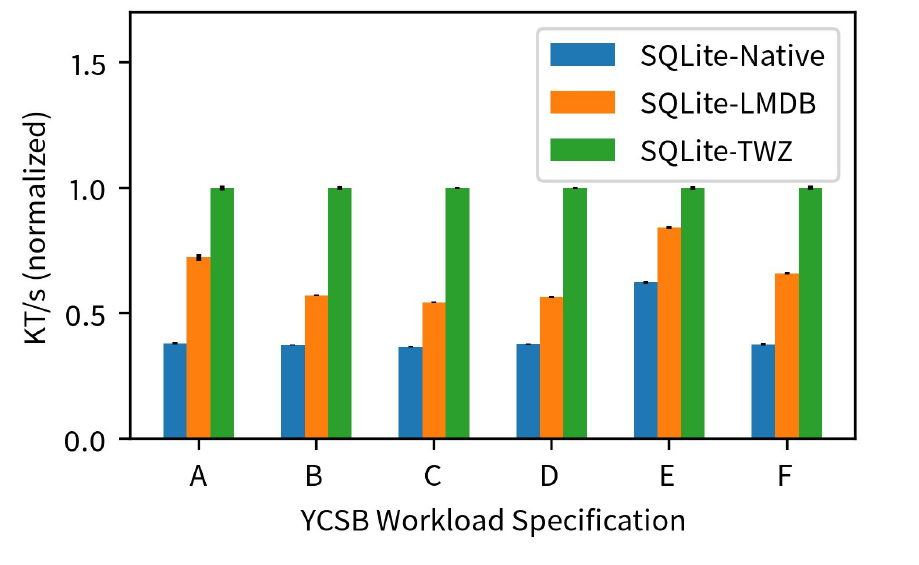
\includegraphics[width=.8\textwidth]{twizzer-sqlite}
    
\end{frame}

%-------------------------------------------------
\begin{frame}
    
    Benchmark: SQLite, latency       
    %    \begin{itemize}
    %        \item                                
    %    \end{itemize}
    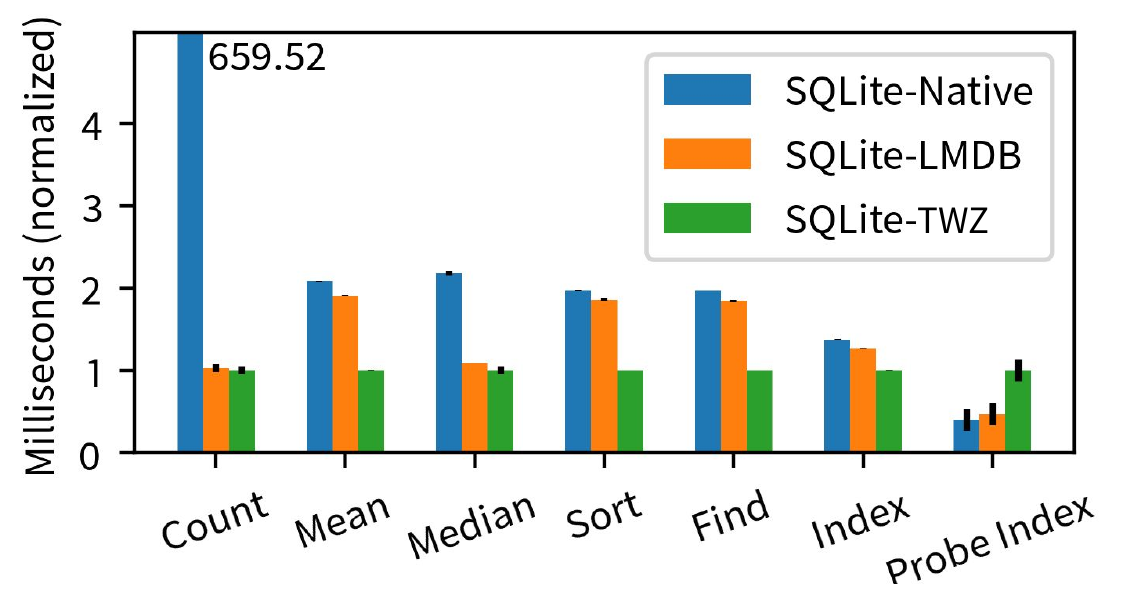
\includegraphics[width=.8\textwidth]{twizzer-sqlite-2}
    
\end{frame}
%-------------------------------------------------
%-------------------------------------------------
\begin{frame}
    
    The Death of the Process
        
    %    \begin{itemize}
    %        \item                                
    %    \end{itemize}
    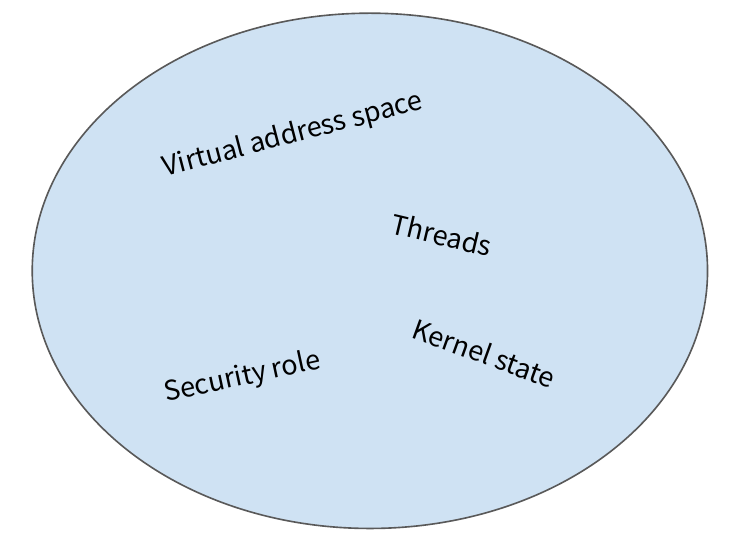
\includegraphics[width=.7\textwidth]{death-of-process}
    
\end{frame}
%-------------------------------------------------
%-------------------------------------------------

\end{document}